\section{What the Server Sees}\label{sec:server}\phantomsection\label{sec:exp-privacy}

The frontier of Sec.~\ref{sec:frontier} counts bytes, not exposure. On exposure, the regimes form a ladder. (i)~\emph{No formal guarantee:} plaintext or PCA uploads (R1), per-party logits (R2), and split learning (R3), which exposes plaintext activations at every step of every epoch and returns gradients to the parties. (ii)~\emph{A formal but loose guarantee:} Gaussian noise added to the upload by each party. (iii)~\emph{Individual vectors hidden:} the ridge head trained under CKKS (R4), which reveals second-order statistics. Local PCA is what makes levels (ii) and (iii) affordable. In Fig.~\ref{fig:frontier}, the best points at which the server receives no plaintext feature are a DP upload after PCA-16 (\dpStSsf\,\% for 512\,B) and the CLIP-L ridge heads under CKKS (up to \heVbCRidgeTf\,\%). We first measure what level (i) reveals.

\subsection{Plaintext uploads are linkable and partly decodable}

\begin{figure}[t]
\centering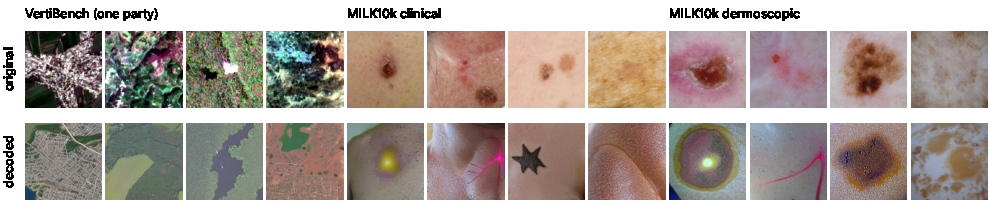
\includegraphics[width=\linewidth]{gen/fig_generic.pdf}
\caption{A public image generator (Stable unCLIP~2.1) applied, without any adaptation, to the CLIP-L uploads of held-out images: the first four attacked test images of VertiBench (one party; contrast-stretched for display) and of MILK10k. It returns an image of the same kind, not the image.}\label{fig:generic}
\end{figure}

\paragraph{Linkage.}
Because the encoder is public, an attacker who holds copies of the candidate images needs no decoder: it encodes them and matches the uploads. Among the \lkN{} VertiBench test images of all parties, the top-1 linkage of CLIP-L uploads is \lkSame\,\% when the attacker reproduces the party's preprocessing, \lkBicubic\,\% after bicubic resizing and \lkEightbit\,\% after 8-bit quantisation, but \lkClip\,\% with CLIP's standard preprocessing. The attack only needs a preprocessing close to the party's.

\paragraph{Decoding.}
Without the images, a public generator decodes part of the content. Stable unCLIP~\cite{ramesh2022unclip,rombach2022ldm}, applied unchanged to VertiBench CLIP-L uploads, returns an image of the same kind of scene, not the image (Fig.~\ref{fig:generic}). An independent encoder (DINOv2-B) picks the source among the \giVbNTest{} test images of the party in \giVbReid\,\% of the cases (top-10: \giVbReidTen\,\%; chance: \giVbChance{} and \giVbChanceTen\,\%). A classifier trained on real images predicts the label from the reconstruction with \giVbLabFone\,\% macro F1, against \giVbRealFone\,\% from the image itself and \giVbChanceFone\,\% by chance. On MILK10k, the decoder draws a lesion-like spot on skin but recovers neither the lesion nor its diagnosis (\giMilkClinLabFone{} and \giMilkDermLabFone\,\% macro F1 for the two modalities, chance \giMilkChanceFone\,\%): what it recovers depends on how well its training images cover the domain. Fine-tuned on public in-domain pairs, the decoder re-identifies no more sources (\giVbBestReid\,\%) and recovers the label only slightly better (\giVbBestLabFone\,\%), while the nearest public image in CLIP space predicts the label as well as the image itself (\giVbNnLabFone\,\%). Decoders trained with a pixel loss on in-domain pairs recover colour, not layout (App.~\ref{app:privacy}). All these attacks bound the leakage from below. We did not attack the pooled DINOv2 token with a generative decoder, nor the activations and features of the trained baselines (SplitNN, FedOnce). Exposure across regimes is therefore compared by what the server receives, not by measured leakage.

\subsection{Party-side transforms and differential privacy}

\paragraph{Secret transforms do not survive a few leaked pairs.}
A party can transform its CLIP-L features before uploading them, with a secret rotation, a private PCA-64, the code of an autoencoder trained on its own features, or a one-layer bottleneck trained by split learning. The attacker then maps the transformed uploads back to CLIP embeddings. Without any image--upload pair of the party, our spectral alignment with public features fails (\gdRotLinkZero\,\% linkage for the rotation). With 100 leaked pairs, i.e.\ 3\,\% of a party's samples, a ridge regression links \gdPcaLinkOneZeroZero{} to \gdAeLinkOneZeroZero\,\% of the uploads for the rotation, the PCA and the autoencoder, and \gdSplitLinkOneZeroZero\,\% for the split bottleneck. Only noise-as-targets codes resist (\gdNatLinkThreeOneFourTwo\,\% with all training pairs), at a cost of \gdNatDrop{} accuracy points (App.~\ref{app:privacy}). A transform that preserves accuracy preserves the information an attacker needs.

\paragraph{Differential privacy is usable after PCA.}
Each party clips its vector, raw or after PCA, at the median norm of its own training vectors and adds isotropic Gaussian noise calibrated to a per-upload $(\varepsilon,\delta{=}10^{-5})$ guarantee by Gaussian DP~\cite{dong2022gdp}. The noise norm grows with the square root of the dimension and the clipped signal does not, so a lower dimension means less noise: PCA is what makes DP usable. At $\varepsilon=8$ per upload, full DINOv2-g features fall to \dpFullEight\,\%, below the majority class (\majVB\,\%), whereas PCA-16 uploads keep \dpStEight\,\%. At $\varepsilon=64$, PCA-16 reaches \dpStSsf\,\% and PCA-64 \dpSfSsf\,\%, against \dpFullSsf\,\% for full features. The guarantee is formal but loose. $\varepsilon$ is per upload, and the 16 uploads of a sample compose to about $\varepsilon\approx50$ for a per-upload $\varepsilon=8$ and $\varepsilon\approx630$ for $\varepsilon=64$, before accounting for the estimation of the clipping norms and of the PCA bases on the training data. The reproduced SplitNN (\reproAcc\,\%) offers no formal guarantee, so DP buys a guarantee, at an accuracy cost.

\subsection{The encrypted point: a ridge head under CKKS}\label{sec:he}

\begin{table}[t]
\caption{Heads that can be trained on encrypted uploads. Accuracy on VertiBench (16 parties) and CIFAR (2 parties), macro F1 on MILK10k and WorldStrat (2 parties); mean\,$\pm$\,std over 5 seeds or folds (CIFAR: 3 seeds). MLP: the reference head, re-run in the same pipeline as the ridge (hence differences of a tenth of a point from Table~\ref{tab:main}). Ridge: closed form from $X^\top X$ and $X^\top Y$ on standardised features (class-weighted on MILK10k and WorldStrat), regularisation chosen on validation, emulated in plaintext; PCA to 256, 64 or 16 components per party; --: Gram matrix too large to emulate (16 parties, full features).}\label{tab:he}
\centering\scriptsize
\setlength{\tabcolsep}{4pt}
\begin{adjustbox}{max width=\linewidth}
\begin{tabular}{@{}lccccc@{}}
\toprule
& \multicolumn{2}{c}{Full features} & \multicolumn{3}{c}{Ridge after per-party PCA}\\
\cmidrule(lr){2-3}\cmidrule(lr){4-6}
Task & MLP & Ridge & 256 & 64 & 16\\
\midrule
\inputtab{gen/tab_he.tex}
\bottomrule
\end{tabular}
\end{adjustbox}
\end{table}

\paragraph{Accuracy.}
With two parties and full features, linearity costs little or nothing on some tasks and a few points on others (Table~\ref{tab:he}): the ridge matches or exceeds the MLP on MILK10k with DINOv2-g (\heMilkGRidgeFull{} vs.\ \heMilkGMlp\,\%) and on WorldStrat IPCC (\heworldstratipccRidgeFull{} vs.\ \heworldstratipccMlp\,\%), but loses on MILK10k with CLIP-L (\heMilkCRidgeFull{} vs.\ \heMilkCMlp\,\%). The encrypted cost, however, grows with the square of the total dimension $D=Kd'$, and 16 full parties are too large even to emulate. After a per-party PCA, the ridge reaches on VertiBench \heVbGRidgeTf{} to \heVbCRidgeTf\,\% with PCA-256, \heVbGRidgeSf{} to \heVbCRidgeSf\,\% with PCA-64 and \heVbGRidgeSt{} to \heVbCRidgeSt\,\% with PCA-16 (DINOv2-g to CLIP-L), against \reproAcc\,\% for plaintext SplitNN. On MILK10k, PCA-64 lowers it to \heMilkGRidgeSf\,\% (DINOv2-g), the level of ResNet-18 split learning from ImageNet weights.

\paragraph{Cost.}
We timed the CKKS operations with TenSEAL on one CPU core (parameters in App.~\ref{app:privacy}). An encrypted inner product of two feature columns takes about \hcVbStCtCt\,ms, and the server needs one per pair of columns from different parties. This amounts to \hcVbStServerH{} core-hours for VertiBench with PCA-16 and \hcVbSfServerH{} with PCA-64. For the class-weighted MILK10k ridge, it amounts to \hcMilkServer{} core-minutes with PCA-64, but about \hcMilkFullH{} core-hours with the full features that its accuracy requires. Encryption also expands each upload \hcVbSfExpand-fold: with PCA-64, a VertiBench party sends \hcVbSfUp{} for its \hcVbSfN{} training samples instead of \hcVbSfPlain{} in half precision, and a MILK10k party with full features sends \hcMilkFullUp. These are operation timings with a single key, and accuracies emulated in plaintext with a measured CKKS error of the order of $10^{-6}$. The collective decryption, the repacking of the aggregates and the end-to-end protocol remain to be implemented. At affordable dimensions, the encrypted ridge therefore scores around or below the plaintext non-foundation reference, and it reveals $X^\top X$ to the server: it is the security end of the frontier, at a cost in accuracy and compute.
